\documentclass[11pt, oneside]{article}   	% use "amsart" instead of "article" for AMSLaTeX format
\usepackage{geometry}                		% See geometry.pdf to learn the layout options. There are lots.
\geometry{letterpaper}                   		% ... or a4paper or a5paper or ...
%\geometry{landscape}                		% Activate for rotated page geometry
%\usepackage[parfill]{parskip}    		% Activate to begin paragraphs with an empty line rather than an indent
\usepackage{graphicx}				% Use pdf, png, jpg, or eps§ with pdflatex; use eps in DVI mode
								% TeX will automatically convert eps --> pdf in pdflatex
\usepackage{amssymb}
\usepackage{hyperref}
\usepackage{amsmath}

\usepackage[scaled]{helvet}
\usepackage[T1]{fontenc}
\renewcommand\familydefault{\sfdefault}

\usepackage{parskip}

\graphicspath{ {./assets/} }

\title{Linear differential equations}
\author{Albert Xu}

\begin{document}
\maketitle

I'm developing an application to \href{https://github.com/alberttxu/diffeqvisualizer}{visualize differential equations}.
The purpose of this app is to help students understand what a differential equation means,
since many college courses don't provide much intuition.
This document covers the mathematics used in the app's demo examples.

\section{Intro}

A differential equation describes a function in terms of its derivatives.
For example, the linear differential equation
\begin{equation} \label{eq:xdoteqAx}
\dot{x} = Ax
\end{equation}
says that a function $x(t)$ must equal its derivative $\dot{x}(t) = \frac{dx}{dt}$ when multiplied by $A$.
The word linear means $\dot{x}$ is expressed in terms of multiplications and additions of $x$.
Basically, there are no $x^2$ or $\sqrt{x}$ terms, additional constant terms, etc.
More generally, a differential equation is defined as $\dot{x} = f(x)$,
but for now we will analyze the linear case.

Important notes:
\begin{itemize}
  \item There are many possible solutions for a differential equation (DE).
  In equation \ref*{eq:xdoteqAx}, $x$ refers to any solution, not necessarily a specific one.
  \item For most complicated DEs there is no closed-form expression that can describe all possible solutions.
  \item For a particular (i.e. specific) solution $x(t)$, it is useful to think of $x$ not as a function, but as some quantity at time $t$ in a simulation.
    \subitem Example: $x$ represents the location of an object, and $\dot{x}$ represents its velocity.
  \item For a particular solution $x(t)$, the set of its past values is sometimes called a trajectory.
  \item The study of a particular solution with a starting value $x_\mathrm{initial}$ at $t = 0$ is called an initial value problem.
\end{itemize}


\section{1-D}

We want to solve equation \ref*{eq:xdoteqAx},
$$\dot{x} = Ax,$$
where $A$, $x$, and $\dot{x}$ are numbers.
Let's use a simple example: $x$ is the location of a particle on a number line and $\dot{x}$ is its velocity.

If $A = 0$ then $\dot{x} = 0$, i.e. velocity is zero for all $x$.
For any initial value of $x$, its trajectory never moves.

If $A > 0$ then trajectories will move away from the origin.
Since $\dot{x}$ is proportional to $x$,
if $x > 0$ the trajectory will move further to the right, and if $x < 0$ it will move further to the left.

If $A < 0$ then trajectories will shrink toward the origin using similar logic.

All 3 cases can be described using the general-form solution,
\begin{equation}
x(t) = ce^{tA} .
\end{equation}
However, for a specific particle, its solution is
\begin{equation} \label{eq:1Dsol}
x(t) = x_\mathrm{initial} e^{tA}
\end{equation}
since $x_\mathrm{initial} = x(0)$ uniquely determines $c$.
\begin{itemize}
  \item Fun fact: this is the same formula used in
  \href{https://en.wikipedia.org/wiki/Compound_interest#Continuous_compounding}{compound interest}.
\end{itemize}

\section{2-D}

This is much more interesting since there are numerous ways a 2-D point can move relative to the origin.
I believe it is very hard to understand the dynamics in this case without a graphical application.
And so I encourage the reader to play around with the elements of $A$ to see how it affects the motion of trajectories.
In the rest of this section I won't go into troublesome formulas and derivations like in most college courses,
and instead only mention basic definitions and notation required to understand this section.
Higher dimensional linear DEs are also known as linear dynamical systems.
An excellent \href{https://see.stanford.edu/Course/EE263}{course} on this topic is taught at Stanford.
And for those who want a quick infographic,
\href{https://en.wikipedia.org/wiki/Stability_theory}{this wikipedia page} has content that supplements the basics covered here,
although in my opinion the language is a bit dense.

In 2 dimensions, $x$ and $\dot{x}$ are vectors with 2 components (a.k.a elements, entries), and $A$ is a $2\times 2$ matrix.
I won't use fancy LaTeX to emphasize that $A$, $x$, and $\dot{x}$ are not scalars.
Equation \ref*{eq:xdoteqAx},
$$ \dot{x} = Ax ,$$
still has the same meaning as before.
We can imagine that $x$ represents a particle's position in a 2-D plane,
and $\dot{x}$ represents its direction of travel (velocity).
$A$ is a map from position to velocity: for a particle at position $x$, its velocity must equal $Ax$ regardless of the time $t$.

The components of $x$ describe its location along individual axes.
For example, $x_1$ is the particle's location in the horizontal direction,
and $x_2$ is its location in the vertical direction.
Likewise $\dot{x}_1$ and $\dot{x}_2$ represent individual velocity components.

If you play around with the entries of $A$ you will see several kinds of behavior:
rotation;
shrinking;
expanding;
approaching seemingly arbitrary axes;
and more.
Here is a screenshot I've taken of the Trajectories demo below.

\begin{figure}[h]
\centering
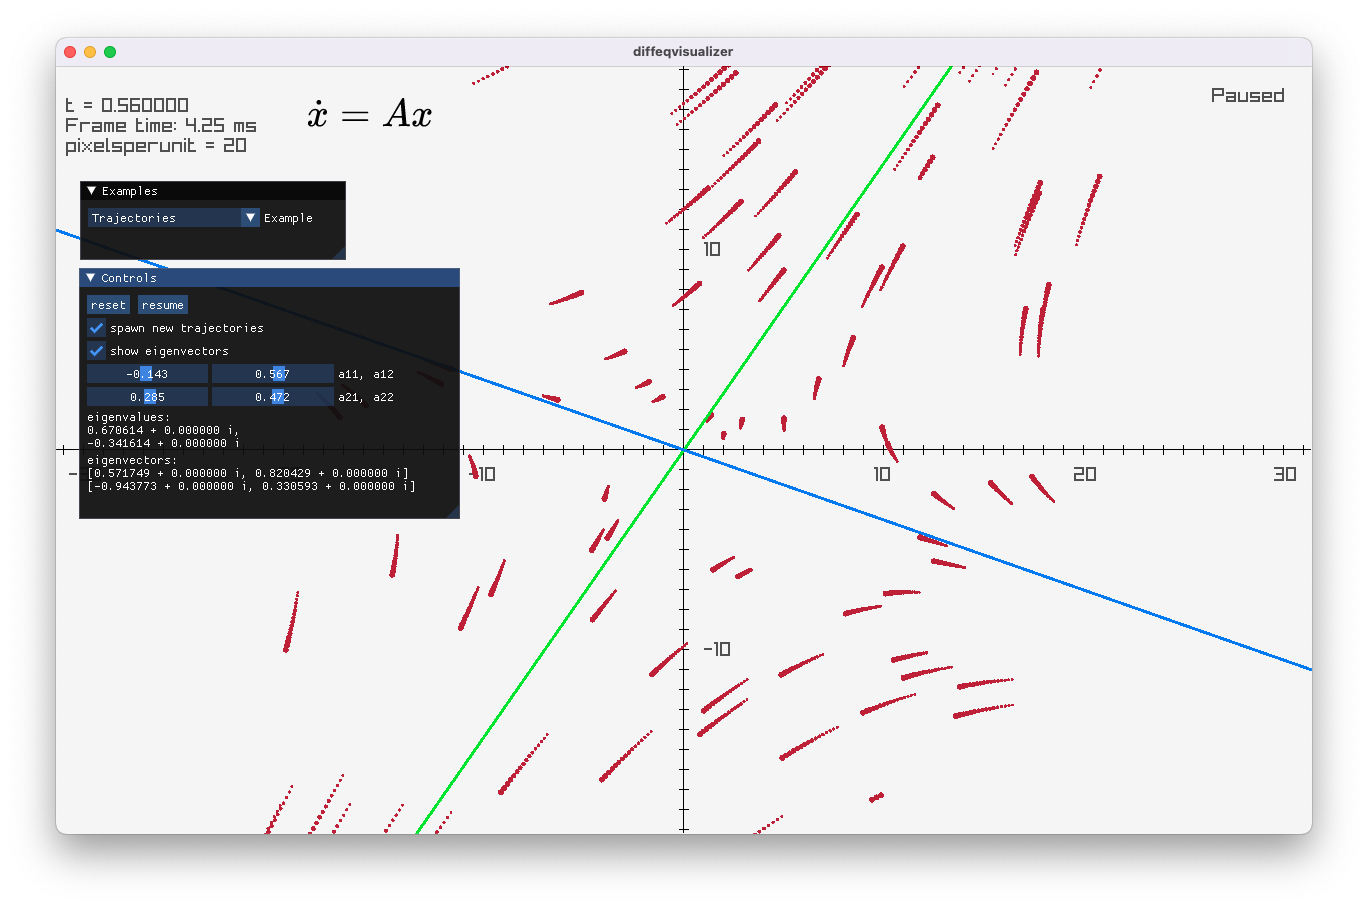
\includegraphics[scale=0.45]{screenshot_trajectories}
\caption{trajectory dynamics of $\dot{x} = Ax$, a.k.a phase space}
\label{fig:Trajectories}
\end{figure}

Each red comet is a trajectory.
You may notice that the trajectories seem to move toward the origin when they are near the blue line,
and are repelled away from the origin near the green line.
This is not a coincidence and it has to do with the eigenvectors of $A$.

\subsection*{Special solution - eigenvector}

An eigenvector of a square matrix, $A$ for example, is a vector $v$ that satisfies the condition
\begin{equation}
Av = \lambda v
\end{equation}
for some $\lambda$.
In the context of our linear DE, $\dot{x} = Ax$, if a trajectory $v$ is an eigenvector of $A$ then
\begin{equation}
\dot{v} = Av = \lambda v
\end{equation}
which is equivalent to two 1-D equations in each entry.
I.e. $\dot{v}_\mathrm{horiz} = \lambda v_\mathrm{horiz}$, $\dot{v}_\mathrm{vert} = \lambda v_\mathrm{vert}$
has the solution $v(t) = e^{\lambda t}v_{\mathrm{initial}}$.
So both of $v$'s components grow or shrink together.
This means that the trajectory $v$ travels either directly towards or away from the origin, but its angle never changes.
$\lambda$ is called the eigenvalue associated with the eigenvector $v$.

Important notes:
\begin{itemize}
\item Any scaled version of $v$ is also an eigenvector of $A$.
Therefore grammatically it is more correct to say $v$ is \textit{an} (instead of \textit{the}) eigenvector associated with $\lambda$.
The line spanned by $v$ is sometimes called the ``eigenspace'' associated with $\lambda$, but this terminology is not universally standard.
\item For an $n\times n$ matrix, there are $n$ eigenvector-eigenvalue pairs. However, the eigenvalues are not necessarily distinct.
\item Conventional notation in many fields denotes eigenvectors as $v_i$ using subscripts.
For example: ``\textit{Let $ v_1,\cdots,v_n $ be eigenvectors of $A$ with associated eigenvalues $ \lambda_1,\cdots,\lambda_n $}.''
Sometimes this is confusing because a subscript is also used to refer to an individual component of a vector.
Be mindful of literary context.
\end{itemize}

\subsection*{General solution}

What if a trajectory $x$ is \textit{not} an eigenvector of $A$?
The insight is that we can break $x$ into pieces which \textit{are} eigenvectors.
That is to say, we can find some scaled eigenvectors $v_1$ and $v_2$ that sum to $x$,
\begin{equation}
x = v_1 + v_2.
\end{equation}
And this separates the dynamics into
\begin{equation}
\dot{x} = Ax
= A(v_1 + v_2)
= A v_1 + A v_2
= \lambda_1 v_1 + \lambda_2 v_2,
\end{equation}
which we can solve because the individual DEs
$$ \dot{v}_1 = A v_1 = \lambda_1 v_1, \quad \dot{v}_2 = A v_2 = \lambda_2 v_2 $$
have solutions
$$ v_1(t) = e^{t\lambda_1}v_{1,\mathrm{initial}}, \quad v_2(t) = e^{t\lambda_2}v_{2,\mathrm{initial}} .$$
Thus, the final solution for $x$ is
\begin{equation}
x(t) = e^{t\lambda_1}v_{1,\mathrm{initial}} + e^{t\lambda_2}v_{2,\mathrm{initial}}
\end{equation}

In summary, we deconstruct $x_\mathrm{initial}$ into $v_{1,\mathrm{initial}}$ \& $v_{2,\mathrm{initial}}$,
scale the individual eigenvectors, and then add the resulting terms to get the solution for $x$.
Hopefully now it is clear what is happening in Figure \ref{fig:Trajectories}.
The eigenvectors of $A$ lie on the blue and green lines.
Those on the blue line have a negative eigenvalue, and those on the green line have a positive eigenvalue.
Each trajectory has components in the blue and green directions.
So over time, the blue component of $x$ shrinks and the green component of $x$ grows.

There is another way to compute the general solution.
You might wonder if we can reuse the formula from the 1-D solution (equation \ref{eq:1Dsol}),
\begin{equation} \label{eq:2Dmatexpsol}
x(t) = e^{tA} x_\mathrm{initial}
\end{equation}
and indeed we can.
Here $e^{tA}$ is a $2\times 2$ matrix --- this is called the matrix exponential function evaluated at $tA$.
But how exactly is it defined?
And how does this method compare to the one based on eigenvectors?
Gilbert Strang has some good answers in this \href{https://youtu.be/LwSk9M5lJx4}{youtube video},
so I won't regurgitate them here.
But I will emphasize what the matrix exponential actually does: it \textbf{acts as a time travel operator}.
Given an initial condition $x_\mathrm{initial} = x(0)$, we can compute a trajectory's future value $x(t)$ for any $t$ (equation \ref*{eq:2Dmatexpsol}).
Furthermore, given a trajectory's current value $x_\mathrm{current} = x(t)$, we can compute its past value from $\Delta t$ seconds \textit{ago}:
\begin{equation}
x(t-\Delta t) = e^{-\Delta t A} x_\mathrm{current}
\end{equation}

See also:
\begin{itemize}
\item 3Blue1Brown has an entire \href{https://youtu.be/O85OWBJ2ayo}{video} dedicated to the matrix exponential.
\item \href{https://www.youtube.com/watch?v=5ePa2UOkEV0&list=PL06960BA52D0DB32B}{Lecture 11} in Professor Boyd's EE263 class
(an essential class for engineering students)
\end{itemize}


\section{Applications}
\subsection*{Harmonic oscillator}

\begin{figure}[h]
\centering
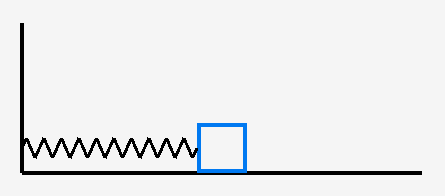
\includegraphics[scale=0.5]{boxspring}
\caption{Box attached to a wall by a spring}
\label{fig:BoxSpring}
\end{figure}

Figure \ref{fig:BoxSpring} shows a box resting at equilibrium.
We would like to analyze the motion of the box if we were to shift it away from equilibrium and then let go.
Let's define our coordinate system with $x = 0$ at the equilibrium position, and $x > 0$ going to the right.
($x$ represents the location of the box's center).

We know from Newton's 2nd law that
\begin{equation} \label{eq:newton2ndlaw}
m \ddot{x} = \sum F_i
\end{equation}
where $F_i$ is any (horizontal) force acting on the box, $m$ is the mass of the box, and $\ddot{x}$ is its acceleration.
We don't include vertical forces since we're analyzing horizontal motion.
There are only 2 forces in this case: the force from the spring, and a friction force from the ground.
The spring force is
\begin{equation}
-k_\mathrm{spring} x
\end{equation}
where $k_\mathrm{spring}$ is a stiffness coefficient.
The spring force always acts towards equilibrium.
The friction force is
\begin{equation}
-k_\mathrm{friction} \dot{x}
\end{equation}
where $k_\mathrm{friction}$ is called the viscous damping coefficient, and $\dot{x}$ is the box's velocity.
The term viscous is used in fluid dynamics, but its the same idea here.
Friction always acts against the direction of velocity because it is a drag force.
With these 2 forces, equation \ref*{eq:newton2ndlaw} becomes
\begin{equation} \label{eq:boxeq}
m \ddot{x} =
-k_\mathrm{spring} x
-k_\mathrm{friction} \dot{x}
\end{equation}
We have not seen this form before.
The $\ddot{x}$ (2nd derivative) term makes this a 2nd-order equation whereas $\dot{x} = Ax$ is a 1st-order equation, so it looks like we are stuck.
The question is whether it is possible to convert equation \ref*{eq:boxeq} into the form $\dot{x} = Ax$.
At this point, some lecturers will pull a ``trick'', and arrive at a new set of equations without explaining why it works.
I'll explain the general method and then apply it to our box-spring system.

\subsubsection*{Converting from higher order to 1st order}

In this subsection $x$ is used in a general context and does not refer to the box's location.
We want to convert a general $n$-th order linear DE of the form
\begin{equation} \label{eq:nthOrderDE}
k_n x^{(n)}
+ k_{n-1} x^{(n-1)}
+ \cdots
+ k_{1} \dot{x}
+ k_{0} x
= 0
\end{equation}
to the familiar form $\dot{x} = Ax$.
The notation $x^{(i)}$ represents the $i$th derivative of $x(t)$ and is equivalent to the dot notation.
The key ``trick'' here is called a \textbf{change of variables}.
We will declare a new vector variable which contains all of the higher derivatives,
and this new variable will satisfy $\dot{x} = Ax$.
Allow me to explain.

Let's declare a variable, $z$, and set it equal to
\begin{align}
z &= \begin{bmatrix}
        x \\
        \dot{x} \\
        \vdots \\
        x^{(n-2)} \\
        x^{(n-1)} \\
      \end{bmatrix}
\end{align}
Then $\dot{z}$ is equal to
\begin{align}
\dot{z} &= \begin{bmatrix}
        \dot{x} \\
        \ddot{x} \\
        \vdots \\
        x^{(n-1)} \\
        x^{(n)} \\
      \end{bmatrix}
\end{align}
which in terms of $z$ is
\begin{align}
\dot{z} &= \begin{bmatrix}
        \dot{x} \\
        \ddot{x} \\
        \vdots \\
        x^{(n-1)} \\
        x^{(n)} \\
      \end{bmatrix}
  =
      \begin{bmatrix}
        0 & 1 & 0 & \dots & 0 \\
        0 & 0 & 1 & \dots & 0 \\
        \vdots & \vdots & \vdots & \ddots & \vdots \\
        0 & 0 & 0 & \dots & 1 \\
        \frac{-k_0}{k_n} & \frac{-k_1}{k_n} & \dots & \frac{-k_{n-2}}{k_n} & \frac{-k_{n-1}}{k_n}
      \end{bmatrix}
      \begin{bmatrix}
        x \\
        \dot{x} \\
        \vdots \\
        x^{(n-2)} \\
        x^{(n-1)} \\
      \end{bmatrix}
  = Az
\end{align}
which is the form $\dot{z} = Az$.
In the first $n-1$ rows of $A$ there is a $1$ located after the diagonal position.
This is a consequence of how we defined $z$ --- the $i$th element of $\dot{z}$ equals the $i+1$th element of $z$.
In the $n$th (last) row the coefficients are the result of isolating $x^{(n)}$ from equation \ref{eq:nthOrderDE} to the left-hand side.
A matrix with this type of pattern is called a companion matrix.

Applying this method to our box-spring system (eq. \ref{eq:boxeq}), we get
\begin{align} \label{eq:boxeqCompanion}
\begin{bmatrix}
        \dot{x} \\
        \ddot{x} \\
      \end{bmatrix}
  =
      \begin{bmatrix}
        0 & 1 \\
        \frac{-k_\mathrm{spring}}{m} & \frac{-k_\mathrm{friction}}{m}
      \end{bmatrix}
      \begin{bmatrix}
        x \\
        \dot{x} \\
      \end{bmatrix}
\end{align}
Let's take a moment to appreciate the simplicity of using linear DEs to analyze this system.
Notice how we didn't need to know any advanced physics, complex analysis, or other prior knowledge.
For instance, take a look at this section of the \href{https://en.wikipedia.org/wiki/Harmonic_oscillator#Universal_oscillator_equation}{Wikipedia page for Harmonic Oscillator}.
There are undefined terms \& symbols, complex exponentials, formulas presented deus ex machina, etc.
In contrast, if you can visualize the dynamics of (\ref*{eq:boxeqCompanion}),
then you already know everything about this oscillator, and can consequently derive the cruft.

\end{document}